\begin{figure}[!htbp]
% \begin{minipage}{6in}
\begin{center}

\begin{minipage}{0.05\textwidth}
~
\end{minipage}%
\begin{minipage}{0.95\textwidth}
\begin{minipage}{0.05\textwidth}
~
\end{minipage}%
\begin{minipage}{0.95\textwidth}
\centering
\large
\textbf{Mean Degree}
\end{minipage}
\begin{minipage}{0.05\textwidth}
~
\end{minipage}%
\begin{minipage}{0.95\linewidth}
\begin{minipage}{0.5\textwidth}
\centering
\large
1
\end{minipage}%
\begin{minipage}{0.5\textwidth}
\centering
\large
2
\end{minipage}
\end{minipage}
\end{minipage}\\
\vspace{2ex}





\begin{minipage}{0.05\textwidth}
\large
\rotatebox[origin=c]{90}{\textbf{Structure}}
\end{minipage}%
\begin{minipage}{0.95\textwidth}
\begin{minipage}{0.05\linewidth}
\large
\rotatebox[origin=c]{90}{Irregular}
\end{minipage}%
\begin{minipage}{0.95\linewidth}
\begin{subfigure}[b]{0.5\textwidth}
\centering
\includegraphics[width=\textwidth]{img/graph_layouts/title=irregular-1+ext=}%
\caption{
Irregular w/ mean degree 1
}
\label{fig:irregular_1}
\end{subfigure}
\begin{subfigure}[b]{0.5\textwidth}
\centering
\includegraphics[width=\textwidth]{img/graph_layouts/title=irregular-2+ext=}%
\caption{
Irregular w/ mean degree 2
}
\label{fig:irregular_2}
\label{fig:irregular_degree_2}
\end{subfigure}

\end{minipage}

\vspace{2ex}

\begin{minipage}{\textwidth}

\begin{minipage}{0.05\linewidth}
\large
\rotatebox[origin=c]{90}{Regular}
\end{minipage}%
\begin{minipage}{0.95\linewidth}
\begin{subfigure}[b]{0.5\textwidth}
\centering
\includegraphics[width=\textwidth]{img/graph_layouts/title=regular-1+ext=}%
\caption{
Regular w/ mean degree 1
}
\label{fig:regular_degree_1}
\label{fig:regular_1}
\end{subfigure}
\begin{subfigure}[b]{0.5\textwidth}
\centering
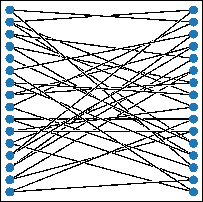
\includegraphics[width=\textwidth]{img/graph_layouts/title=regular-2+ext=}%
\caption{
Regular w/ mean degree 2
}
\label{fig:regular_degree_2}
\label{fig:regular_2}
\end{subfigure}
\end{minipage}
\end{minipage}
\end{minipage}

\caption{
Example target graph layouts used in 32-node graph-matching evolutionary experiments.
Blue dots represent tagged nodes.
Black lines represent selected-for tight affinity relationships.
Layouts differ in total number of selected-for affinities (``mean degree'') and whether selected-for affinities were evenly or randomly distributed between nodes (``structure'').
}
\label{fig:graph_layouts}


\end{center}
% \end{minipage}
\end{figure}
